\chapter{Related Literature}
\begin{quote} 
\textit{ **This chapter reviews the relevant literature's to establish the research context necessary for the thesis.** OR **This section explores contemporary academic/scientific papers and research that forms the basis for this thesis. ** } 
\end{quote}


  
\section{Dye-Sensitized Solar Cells(DSCs)}

**Move part of the text and pictures from introduction to here **


\subsection{Single diode model}\label{SDM}
 \begin{figure}[H]
  \begin{center}
  
\includegraphics[width=\textwidth]{images/pacehold}
  \caption{ Single diode model for a solar cell }
  \label{fig:EQu_cell}
  \end{center}
  \end{figure}

\subsection{Double diode model}\label{DDM}
 \begin{figure}[H]
  \begin{center}
  
\includegraphics[width=\textwidth]{images/pacehold}
  \caption{ Double diode model for a solar cell }
  \label{fig:Double_EQu_cell}
  \end{center}
  \end{figure}
\subsection{Equivalent DSCs model}

\subsection{**Text**\cite{wenger2010strategies}}

Wenger, Sophie.- "\textit{Strategies to optimizing dye-sensitized solar cells: organic sensitizers, tandem device structures, and numerical device modeling}". Diss. ÉCOLE POLYTECHNIQUE FÉDÉRALE DE LAUSANNE, 2010.\\

Solar energy can be converted into electricity by a variety of technologies that can be divided into four classes: Concentrator systems, wafer-based crystalline silicon, thin-film technologies, and emerging technologies. 

  \begin{figure}[H]
  \begin{center}
  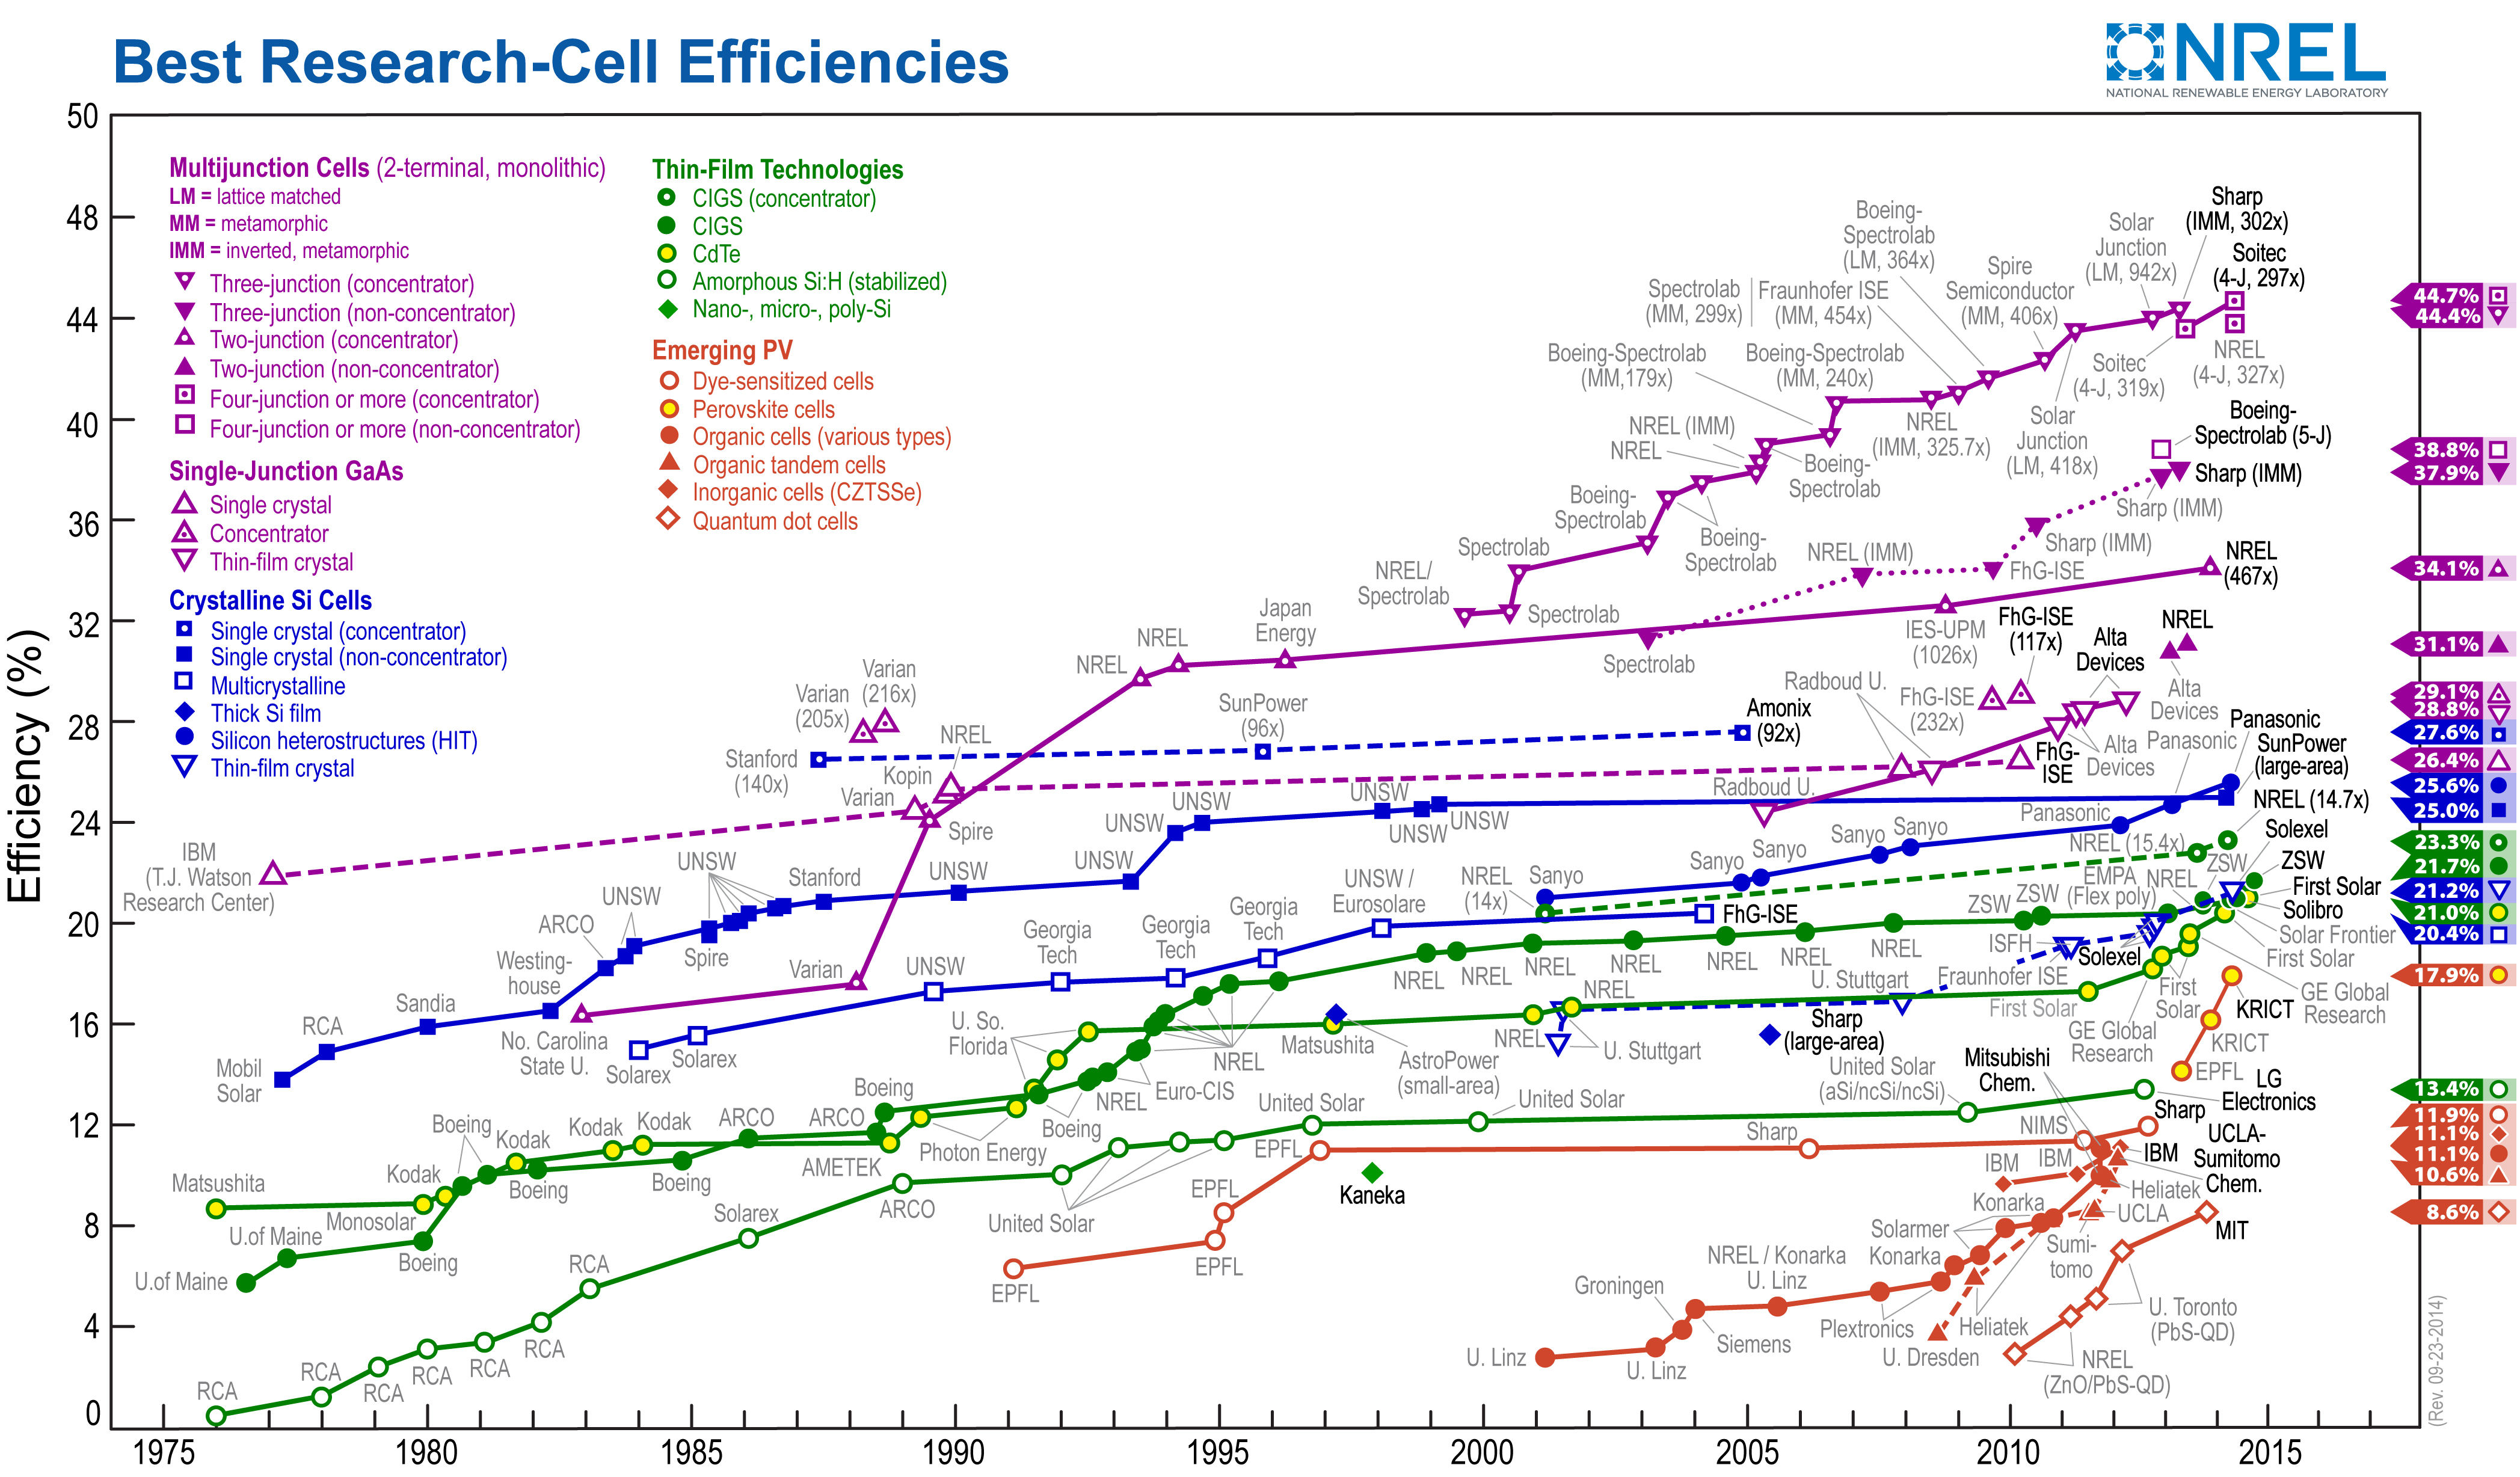
\includegraphics[width=\textwidth]{images/efficiency_chart.jpg}
  \caption{Research Cell Efficiency Records \cite{nrel_Research_Cell} }
  \label{fig:Cell_eficency}
  \end{center}
  \end{figure}


The power conversion efficiency of a solar cell is determined from the current versus applied voltage (I-V ) characteristics under illumination. The I-V curve and device efficiency are reported with respect to a standard reference spectral irradiance distribution, the air mass 1.5 global (AM 1.5G) spectrum. The I-V characteristics of a solar cell are well described by an equivalent electric circuit in Figure ~\ref{fig:EQu_cell} on page ~\pageref{fig:EQu_cell} . Under illumination, a constant photo current (I\textsubscript{ph}) is generated.If a forward voltage bias is applied, a dark diode current (I\textsubscript{dark}) flows in the opposite direction. A shunt resistance (R\textsubscript{shunt}) may arise from charge recombination in the photo-active layer and induce a shunting current(I\textsubscript{shunt}).The series resistance (R\textsubscript{series}) includes the contact resistance at interfaces, the bulk resistance, and the sheet resistance of the transparent electrodes. The total measured current then is
 
 \begin{equation}
 \begin{aligned}
  I = I\textsubscript{ph} - I\textsubscript{dark} - I\textsubscript{shunt} = I\textsubscript{ph} -  I\textsubscript{s} (e^{\frac{eV}{\textit{mk}T}-1}) - \dfrac{V+IR\textsubscript{series}}{R\textsubscript{shunt}}
   \label{eq:equ_current}
   \end{aligned}
   \end{equation}

 where \textbf{I\textsubscript{s}} is the diode saturation current, \textbf{V} is the applied bias voltage, \textbf{\textit{m}} is an ideality factor ( \textit{m} = 1 for an ideal cell), \textbf{\textit{k}} is the Boltzmann constant, and \textbf{T} is the device temperature\cite{pointwenger2010strategies}.
  
 

The maximum-power operating point defines the condition at which the power output (P\textsubscript{\textit{max}} = I\textsubscript{\textit{max}}V\textsubscript{\textit{max}}) of the device is maximal.
The so-called \ac{F.F} is often used to characterize the maximum power ,

\begin{equation}
 \begin{aligned}
  \ac{F.F} = \dfrac{I\textsubscript{\textit{max}}V\textsubscript{\textit{max}}}{I\textsubscript{\textit{sc}}V\textsubscript{\textit{oc}}}
   \label{eq:equ_current}
   \end{aligned}
   \end{equation}

**Pictures and text about losses in the light absorption in the cell **

**talk ABOUT STABILITY OF dcs with change in temperature **

\section{Maximum power Point Tracking(MPPT)}

**some points form the Introduction can be moved here like the methods of MPP control Algo etc ** \\

Despite all the advantages presented by the generation of energy through the use of PVs, the efficiency of energy conversion is currently low and the initial cost for its implementation is still considered high, and thus it becomes necessary to use techniques to extract the maximum power from these panels, in order to achieve maximum efficiency in operation. It should be noted that there is only one maximum power point (MPP), and this varies according to climatic and irradiation conditions\cite{eltawil2013mppt}.

To overcome this problem, several methods for extracting the maximum power have been proposed in literature **citations **

\subsection{**text**\cite{ngan2011study}}

Ngan, Mei Shan, and Chee Wei Tan. "\textit{A study of maximum power point tracking algorithms for stand-alone photovoltaic systems.}" Applied Power Electronics Colloquium (IAPEC), 2011 IEEE. IEEE, 2011. \\

**Text about the paper **

\subsection{**text**\cite{ngan2011study}}

Ngan, Mei Shan, and Chee Wei Tan. "\textit{A study of maximum power point tracking algorithms for stand-alone photovoltaic systems.}" Applied Power Electronics Colloquium (IAPEC), 2011 IEEE. IEEE, 2011. \\

**Text about the paper **

\subsection{**text**\cite{esram2007comparison}}

Esram, Trishan, and Patrick L. Chapman. "\textit{Comparison of photovoltaic array maximum power point tracking techniques.}" IEEE TRANSACTIONS ON ENERGY CONVERSION EC 22.2 (2007): 439.\\

**almost all the Work in eltawil2013mppt is derived from this paper including pictures and text **
 
\subsection{**text**\cite{eltawil2013mppt}}

Eltawil, Mohamed A., and Zhengming Zhao. "\textit{MPPT techniques for photovoltaic applications.}" Renewable and Sustainable Energy Reviews 25 (2013): 793-813. \\

This article aims to assess different MPPT techniques, provide background knowledge, implementation topology, grid interconnection of PV and solar microinverter requirements presented in the literature, doing in depth comparisons between them with a brief discussion. The MPPT merits, demerits and classification, which can be used as a reference for future research related to optimizing the solar power generation, are also discussed.\\

**Text about the paper **

\subsection{**text**\cite{reza2013classification}}

Reza Reisi, Ali, Mohammad Hassan Moradi, and Shahriar Jamasb. "\textit{Classification and comparison of maximum power point tracking techniques for photovoltaic system: A review.}" Renewable and Sustainable Energy Reviews 19 (2013): 433-443.

\subsection{**text**\cite{faranda2008energy}}

Faranda, Roberto, and Sonia Leva. "\textit{Energy comparison of MPPT techniques for PV Systems.}" WSEAS transactions on power systems 3.6 (2008): 446-455.\\

This paper presents a comparative study of ten widely-adopted MPPT algorithms; their performance is evaluated on the energy point of view, by using the simulation tool Simulink{\textregistered}, considering different solar irradiance variations.\\

My thesis borrows some of the algorithms/Flow Chart mentioned in the above four papers. 

\subsection{**text**\cite{houssamo2013experimental}}

Houssamo, Issam, Fabrice Locment, and Manuela Sechilariu. "\textit{Experimental analysis of impact of MPPT methods on energy efficiency for photovoltaic power systems.}" International Journal of Electrical Power \& Energy Systems 46 (2013): 98-107.\\

This work presents an experimental comparison; Using four identical PV, under strictly the same set of technical and meteorological conditions, an experimental comparison  of four most used MPPT methods for PV power systems is done.This comparison shows the advantage of use of a MPPT with a variable tracking step.\\  

\subsection{**text**\cite{jain2004new}}
Jain, Sachin, and Vivek Agarwal. "\textit{A new algorithm for rapid tracking of approximate maximum power point in photovoltaic systems.}" Power Electronics Letters, IEEE 2.1 (2004): 16-19.\\

This paper presents a new algorithm for tracking maximum power point in photovoltaic systems. This is a fast tracking algorithm, where an initial approximation of \ac{MPP} quickly achieved using a variable step-size. Subsequently, the exact\ac{MPP} can be targeted using any conventional method like the hill-climbing or incremental conductance method. Thus, the drawback of a fixed small step-size over the entire tracking range is removed, resulting in reduced number of iterations and much faster tracking compared to conventional methods. \\

My implementation draws inspiration for the above article for its  two-stage algorithm to reduce the number of iterations but deviates significantly in the implementation and algorithms used to identify the \ac{MPP} 

\subsection{**text**\cite{liu2011fast}}

Liu, Yi-Hua, and Jia-Wei Huang. "\textit{A fast and low cost analog maximum power point tracking method for low power photovoltaic systems.}" Solar Energy 85.11 (2011): 2771-2780.\\

**add TEXT important RESEARCH * \\

Typically, MPPT methods utilized in medium and high power PV systems uses measured cell characteristics (current, voltage, power) along with an online search algorithm to compute the corresponding \ac{MPP}. Due to the complexity of the required mathematical operations, a \ac{DSP} or a relatively powerful micro-controller is typically needed, which increases the cost of the system.Moreover, it consumes significant portion of the generated power. Therefore, a\ac{MPPT} circuit with low-cost and fast-tracking features is essential .\\

It has already established that there exists a relation between V\textsubscript{MPP} and V\textsubscript{OC} in equation ~\ref{eq:equ_fracoc} and is famously used in the \ac{FOCV} method. However we see that this does not hold true for all illumination conditions and certainly not for low-light(less than ~1500 Lux ) as compared to higher insolation. Since V\textsubscript{OC} is is a logarithmic function of I\textsubscript{ph}, the relationship between  V\textsubscript{MP} and I\textsubscript{MP}.with respect to irradiation is not linear. However, it is possible to linearize this relationship for an interval where the value of V\textsubscript{OC} is sufficiently insensitive to irradiation. That is, the  \ac{VAL} can be calculated as the tangent line of the \ac{MPP} locus where the sensitivity of V\textsubscript{OC} to I\textsubscript{ph} is lower than a pre-defined threshold. This relationship is illustrated in Figure ~\ref{fig:Lui_IV_1} on page ~\pageref{fig:Lui_IV_1}.


 \begin{figure}[H]
  \begin{center}
  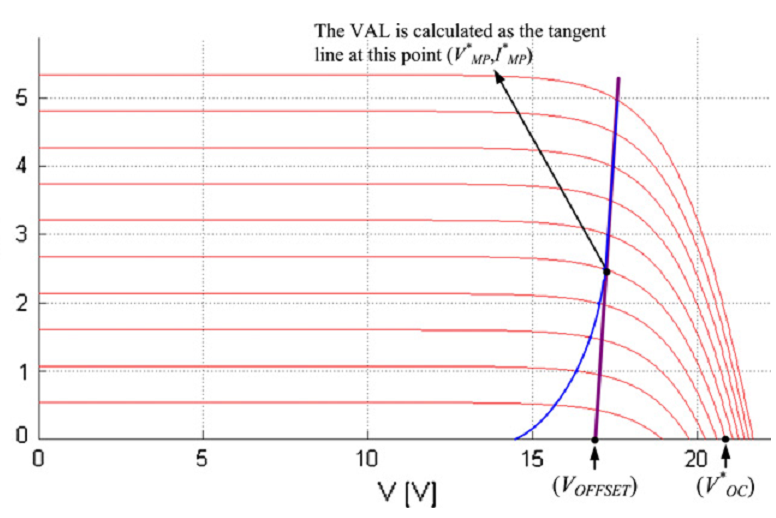
\includegraphics[width=\textwidth]{images/IVCurve_lui}
  \caption{I–V curves of the solar panel under different irradiation levels and the voltage approximation line. \cite{liu2011fast} }
  \label{fig:Lui_IV_1}
  \end{center}
  \end{figure}
  
  The same trend can be seen on the I-V curves for the \ac{DSCs} under test (Figure ~\ref{fig:vmmp_lux50_5000}).
   \begin{figure}[H]
    \begin{center}
    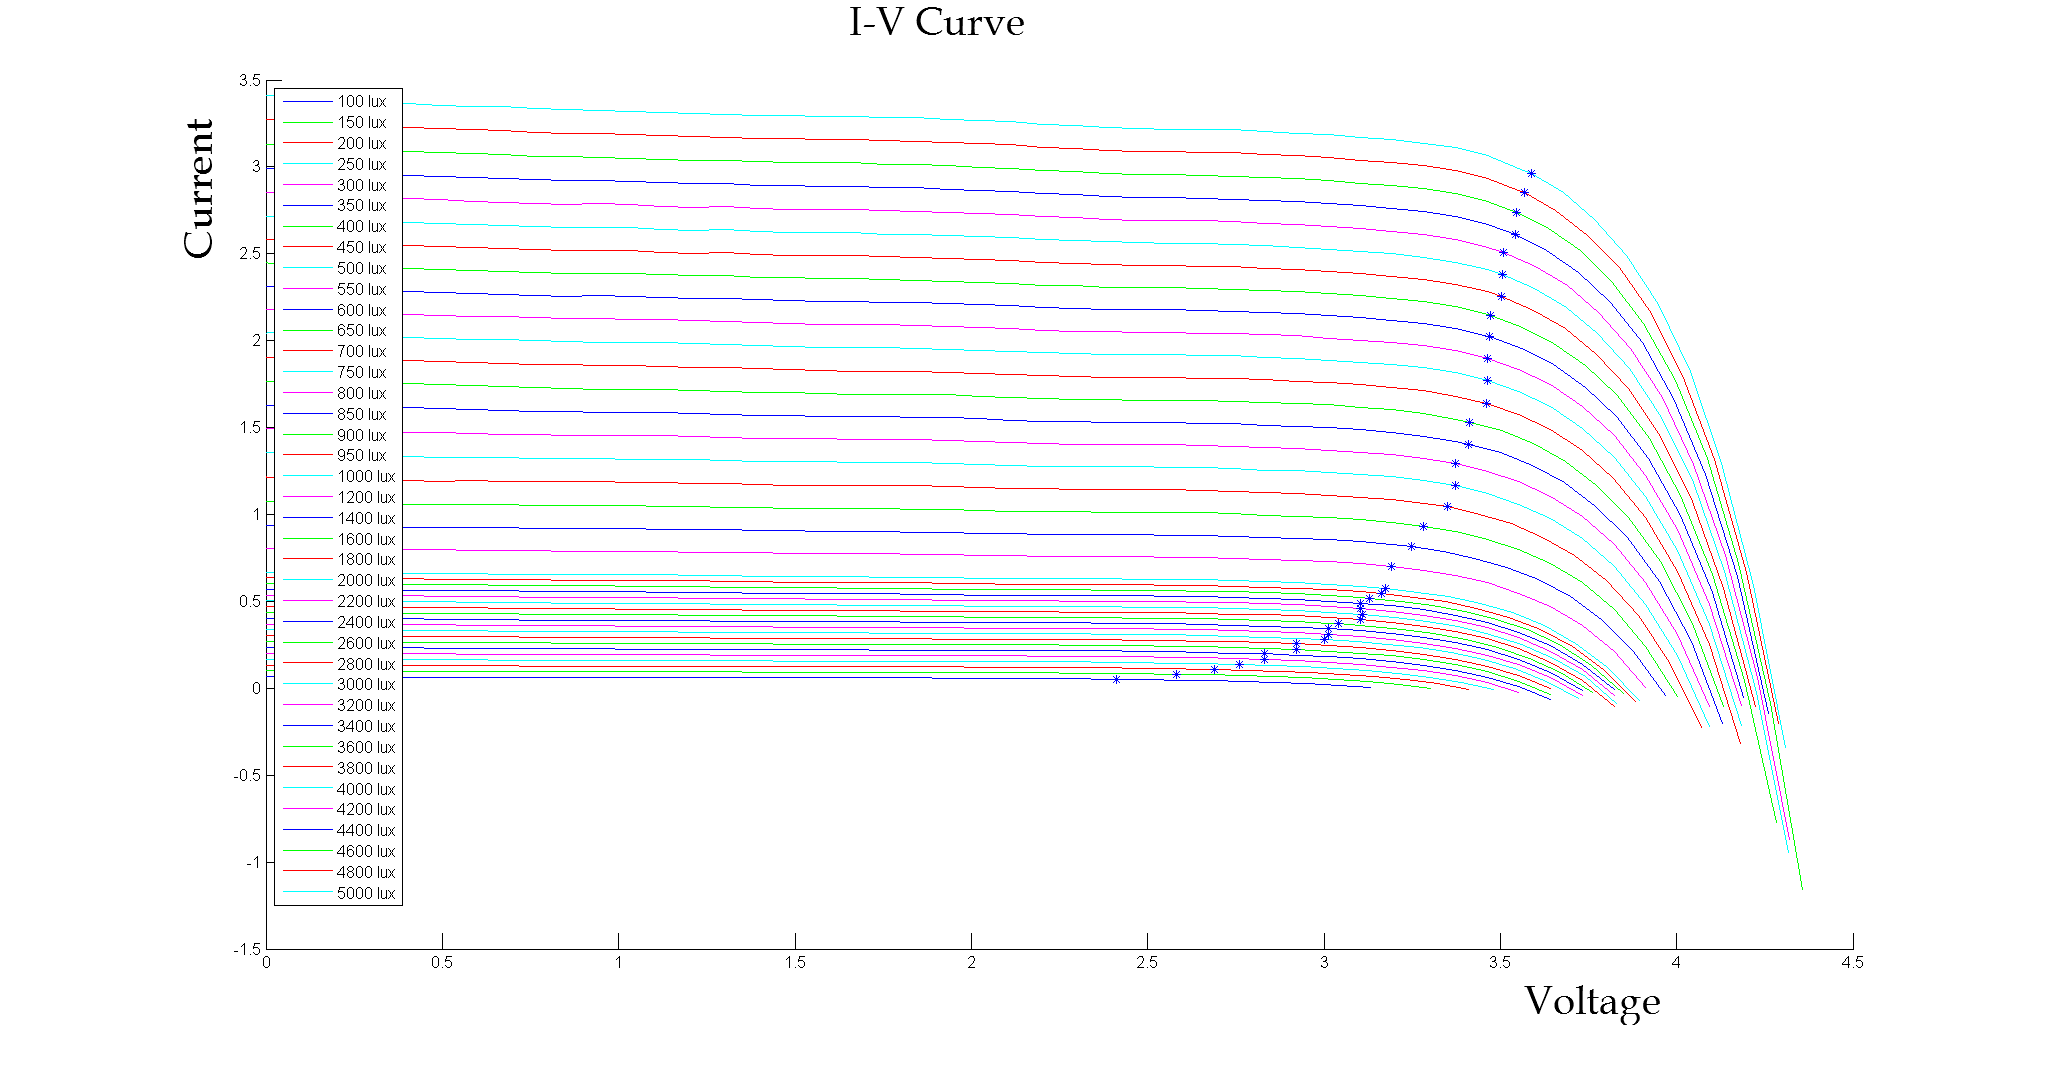
\includegraphics[width=\textwidth]{images/IV_50-500}
    \caption{Variation of V\textsubscript{MPP} for different illumination observed **in/on** the DSC under test }
    \label{fig:vmmp_lux50_5000}
    \end{center}
    \end{figure}
  

 \begin{figure}[H]
  \begin{center}
  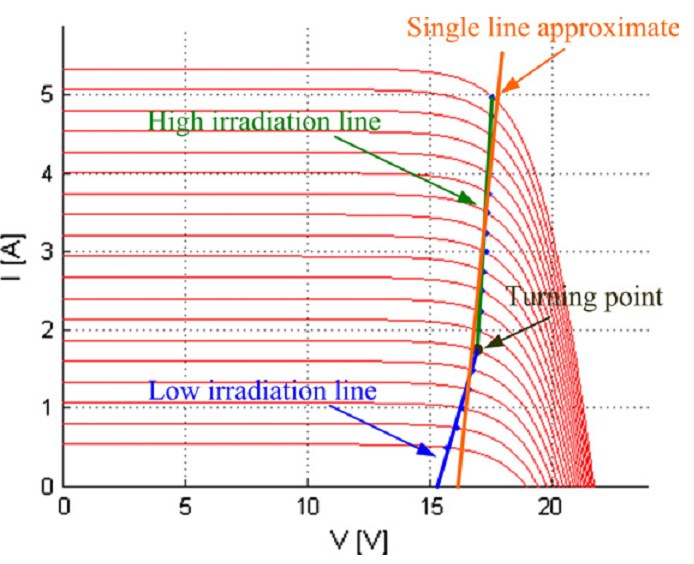
\includegraphics[width=\textwidth]{images/IVCurve_lui_2}
  \caption{Research Cell Efficiency Records \cite{liu2011fast} }
  \label{fig:Lui_IV_2}
  \end{center}
  \end{figure}





**insert pictures**

\subsection{**text**\cite{dondi2008modeling}}

Dondi, Denis, et al. "\textit{Modeling and optimization of a solar energy harvester system for self-powered wireless sensor networks.}" Industrial Electronics, IEEE Transactions on 55.7 (2008): 2759-2766.\\


**Initial modelling strategies where based on this paper,  improving the efficiency. \# discrete components\# ** 

\subsection{**text**\cite{chu2009robust}}
Chu, Chen-Chi, and Chieh-Li Chen. "\textit{Robust maximum power point tracking method for photovoltaic cells: A sliding mode control approach.}" Solar Energy 83.8 (2009): 1370-1378.\\

\subsection{**text**\cite{urayai2011single}}
Urayai, Caston, and G. Amaratunga. "\textit{Single sensor boost converter-based maximum power point tracking algorithms.}" Applied Power Electronics Conference and Exposition (APEC), 2011 Twenty-Sixth Annual IEEE. IEEE, 2011.\\

Two new maximum power point tracking algorithms are presented: the input voltage sensor, and duty ratio maximum power point tracking algorithm (ViSD algorithm); and the output voltage sensor, and duty ratio maximum power point tracking algorithm (VoSD algorithm).unlike the incremental conductance algorithm which requires two sensors (the voltage sensor and current sensor), the two algorithms are more desirable because they require only one sensor: the voltage sensor.  \\ 

\subsection{**text**\cite{clark2006power}}

Clark, C., and A. Lopez. "\textit{Power system challenges for small satellite missions.}" Proceedings of the 2006 Small Satellites, Systems and Services Symposium, D. Danesy, Ed. The Netherlands: ESA. 2006.\\


**TExt**
Inspiration for use of multiple power buses 



\section{Machine Learning ???}
This section discusses about Search optimization in order to lock on the  V\textsubscript{MP} and I\textsubscript{MP} as efficiently as possible.

\subsection{Regression Modelling \cite{lenarreg2006}}

We use regression analysis when we want to predict one variable from another. The most basic form of regression is called simple regression, where We have 1 independent variable and 1 dependent variable and where we are predicting a linear trend. In regression, we attempt to determine the magnitude of the relationship between a set of independent variables and the dependent variable. Independent variable(X), Also called the predictor variable, that we believe influences our Dependent variable(Y),Also called the response variable.\\

A regression model is a formal way of stating:
\begin{itemize}
\item The tendency of the response variable(Y) to vary with the predictor variable(X).
\item A scattering of points around some statistical relationship.
\end {itemize}

Equation for a line can be written as:

\begin{equation}
\begin{aligned}
  y= mx + b 
\label{eq:Line_equ}
\end{aligned}
\end{equation}

The linear regression model(for observation i = 1, . . . , N) can we written as:

\begin{equation}
\begin{aligned}
  Y\textsubscript{i}= \beta\textsubscript{0}+\beta\textsubscript{1}X\textsubscript{i} +\epsilon\textsubscript{i}
\label{eq:Line_equ}
\end{aligned}
\end{equation}

\begin{itemize}
\item $\beta\textsubscript{0}$ is the mean of the population when X is zero -the Y intercept.\\
\item $\beta\textsubscript{1}$ is the slope of the line, the amount of increase in Y brought about by a unit increase $(X^{'}= X + 1)$ in X.\\
\item \textbf{$\epsilon\textsubscript{i}$} is the random error, specific to each observation.
\end {itemize}



**add more text about line Linear Regression **


\subsection{Pattern search}

Seiler, Mary C., and Fritz A. Seiler. "\textit{Numerical recipes in C: the art of scientific computing.- 10.2 Golden Section Search in One dimention}" Risk Analysis 9.3 (1989): 415-416.\\

Finding the Maxima or minima of a first order single variable function can easily be found by equating the derivative of this function to zero. However finding the derivative of certain functions is not always easy or possible.In such conditions Search techniques are used to find the Maxima or minima in a uni-modal((A uni-modal function contains only one minimum or maximum on the specified interval ) continuous function over an interval without using derivatives.  Golden Section search Algorithm is one such search method. The Algorithm derives its name from the Golden ratio(0.61803...)\\

Two numbers are said to be in the golden ratio if their ratio is same as the ratio of their sum to the larger of the two quantities.Assuming b > a then this can be expressed as:\\

\begin{equation}
\begin{aligned}
 \dfrac{a+b}{b}=\dfrac{b}{a}=\phi
\label{eq:golden_ratio1}
\end{aligned}
\end{equation}

where ${\phi}$ is the golden ratio whose value is given by:\\

\begin{equation}
\begin{aligned}
 \phi=\dfrac{\sqrt{5}-1}{2}= 0.61803398874989......
\label{eq:golden_ratio}
\end{aligned}
\end{equation}
**add more text about Golden search **
\begin{figure}[H]
  \begin{center}
  
\includegraphics[width=\textwidth]{images/pacehold}
  \caption{ Golden Section search Algorithm }
  \label{fig:Golden_search}
  \end{center}
  \end{figure}